\section{Quantum Distribution Key (QDK)}
E' un modo alternativo al DH per lo scambio di chiavi.
Permette di scambiare lunghe chiavi da utilizzarsi con one-time pad.
Inoltre è già utilizzato in quanto non necessita dell'utilizzo di computer quantistici e se in futuro la tecnologia quantistica dovesse evolversi comunque questo protocollo sarebbe quantistico-resistente oltre che resistente al collasso della classe NP.

Questo protocollo inoltre permette di accertare una eventuale intrusione, eventualmente si butta via la chiave, proprio per questo motivo non si puà usare per scambiare messaggi.

NB: esiste poi la crittografia post-quantistica che si occupa di cercare sistemi a chiave pubblica inattaccabili anche da macchine quantistiche.
Ci si basa su problemi NP-completi che si sanno essere difficili anche con una eventuale supremazia quantistica.

Es: Grover è un algoritmo quantistico che permette di risolvere problemi NP-completi ma sempre on O($s^{\frac{n}{2}}$) quindi sub-esponenziale.
Un esempio di sistema quantistico-resistente è quello su reticoli.

Sfruttiamo i seguenti principi della meccanica quantistica:
\begin{itemize}
    \item \emph{sovrapposizione degli stati}: un sistema quantistico si può trovare in più di uno stato allo stesso tempo
    \item \emph{decoerenza}: quando si effettua una misurazione il sistema si \emph{perturba} quindi collassa solo in uno degli stati che prima erano sovrapposti.
    Si lascia quindi una traccia all'atto della misurazione, la usiamo per controllare circa eventuali intromissioni nella trasmissione
    \item \emph{no-cloning}: impossibilità di fare una copia di un sistema quantistico.
    Per copiare bisogna misurare, ma misurare significa modificare il sistema e quindi lasciare una traccia
    \item \emph{entanglement}: la possibilità che due sistemi creati con una correlazione tra loro continuino a mantenere la correlazione anche se portati a grandi distanze l'uno dall'altro (al contrario del principio di località della fisica classica).
    Quindi una misura eseguita su uno dei due influenza anche lo stato dell'altro seppur a larghissima distanza.
\end{itemize}

\subsection{Protocollo BB84}
Nasce nel 1984 da Bennet e Brassard.
Si fa tramite lo scambio di \emph{fotoni polarizzati}.
Ogni fotone ha varie proprietà, tra le quali il \emph{piano di polarizzazione}, consideriamo 4 stati di polarizzazione:

\begin{figure}[H]
    \centering
    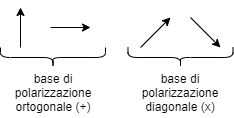
\includegraphics[width=150px]{QDK_1.png}
\end{figure}

La direzione di polarizzazione può essere qualsiasi quindi scegliamo una base per rappresentarla (come se fosse un vettore).
In ognuno di questi stati codifichiamo un bit:
\begin{itemize}
    \item verticale: 0
    \item orizzontale : 1
    \item +45°: 0
    \item -45°: 1
\end{itemize}

NB: Perché due basi? Se ne usassimo una sola potremmo misurare perfettamente lo stato, se invece non so quale base abbiamo usato non posso effettuare misurazioni corrette e certe ma solo probabilistiche, noi ci basimo proprio su questa probabilità!

Vediamo la struttura generale dell' hardware necessario:

\begin{figure}[H]
    \centering
    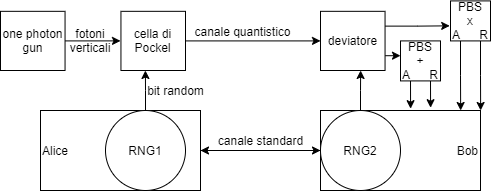
\includegraphics[width=300px]{QDK_2.png}
\end{figure}

Ci si muove su due canali, uno quantistico (fibra ottica) ed uno standard. Solo uno dei due trasmette sul quantistico. Si utilizzano:
\begin{itemize}
    \item One Photon Gun: emette singoli fotoni tutti verticali
    \item Cella di Pockel: impone una determinata polarizzazione scelta dal RNG1
    \item PBS (beam splitter polarizzante): ci da corretta polarizzazione del fotone se e solo se la base di generazione e la base di misurazione sono le stesse. Misura il fotone tramite la deviazione verso una delle due uscite: A (assorbimento) ed R (riflessione).
    Quando il fotone esce, esce con una delle due polarizzazioni misurabili dal PBS, non importa più quella originale.
\end{itemize}

Sia $\theta$ l'angolo tra la base di polarizzazione di misurazione e la polarizzazione del fotone stesso, allora si hanno:
\begin{itemize}
    \item esce da A con probabilità $cos^2 \theta$
    \item esce da R con probabilità $sin^2 \theta$
\end{itemize}

Si noti quindi che:
\begin{itemize}
    \item se la base di misurazione e la base di generazione sono identiche il fotone mantiene la polarizzazione
    \item se le basi di misurazione e di generazione sono diverse $\theta = \pm45^{\circ}$ quindi $cos^2\theta = sin^2\theta = \frac{1}{2}$ quindi il fotone ha pari probabilità di uscire da A o da R.
\end{itemize}

La lettura attraverso il PBS quindi potrebbe distruggere lo stato quantistico precedente:
\begin{table}[ht!]
    \centering
    \begin{tabular}{c|c|c|c|c}
        & 0 $\uparrow$ & 0 $\nearrow$ & 1 $\rightarrow$ & 1 $\searrow$ \\
        \hline
        + & $\uparrow$ & $\uparrow \rightarrow$ & $\rightarrow$ & $\uparrow \rightarrow$  \\
        x & $\nearrow \searrow$ & $\nearrow$ & $\nearrow \searrow$ & $\searrow$
    \end{tabular}
\end{table}

Andiamo dunque al protocollo:
\begin{itemize}
    \item Alice si segna le basi usate per generare i fotoni: $S_A$
    \item Bob si segna quali basi ha usato per effettuare le misure: $S_B$
    \item Bob invia ad Alice le sue basi (sul canale standard)
    \item Alice risponde dicendo quali basi sono corrette
    \item Dove le basi sono concordi si prendono i bit, dove le basi sono discordi si buttano.
    Si ha circa il 50\% di match
\end{itemize}

In assenza di interferenze di Eve, Alice e Bob possiedono $S_A' = S_B'$ sottosequenze identiche formate dai bit codificati e decodificati con basi comuni:
$$ \mid S_A' \mid = \mid S_B' \mid = \frac{\mid S_A \mid}{2} $$

\begin{table}[ht!]
    \centering
    \begin{tabular}{c|c c c c c c c c | c}
        Alice: & 1 & 0 & 1 & 1 & 1 & 0 & 0 & ... & $S_A$ \\
        Alice: & + & x & + & x & x & + & x & ... & basi di A \\
        invia: & $\rightarrow$ & $\nearrow$ & $\rightarrow$ & $\searrow$ & $\searrow$ & $\uparrow$ & $\nearrow$ & ... & fotoni di A \\
    
        & & & & & & & & & \\

        Bob: & + & x & + & + & + & x & x & ... & basi di B \\
        Bob: & $\rightarrow$ & $\nearrow$ & $\rightarrow$ & $\uparrow$ 50\% & $\rightarrow$ 50\% & $\searrow$ 50\% & $\nearrow$ & ... & letture di B \\
        Riceve: & 1 & 0 & 1 & 0 & 1 & 1 & 0 & ... & $S_B$ \\
    \end{tabular}
\end{table}

Le basi concordi sono 1, 2, 3, 7 che portano alla sequenza:
$$ S_A' = S_B' = 1010 $$

Se c'è un crittoanalista esso si troverà nella stessa situazione di Bob, quindi deve scegliere le sue basi.
Le basi che sceglierà saranno indipendenti da quelle di Alice e Bob quindi se la sua base coincide con quella di Alice non cambia nulla, invece se non coincide altera irreparabilmente il fotone!
Alice e Bob fanno quindi una verifica: sacrificano un pezzo si $S_A'$ e $S_B'$:
si scambiano una porzione delle chiavi comuni in posizioni prestabilite comunicandole sul canale standard.
Se le due sequenze sono diverse allora interrompono la comunicazione.
Altrimenti usano la porzione rimanente come chiave o per costruire la chiave.


\begin{table}[ht!]
    \centering
    \begin{tabular}{c|c c c c c c c c}
        Alice: & 1 & 0 & 1 & 1 & 1 & 0 & 0 & ... \\
        Alice: & + & x & + & x & x & + & x & ... \\
        invia: & $\rightarrow$ & $\nearrow$ & $\rightarrow$ & $\searrow$ & $\searrow$ & $\uparrow$ & $\nearrow$ & ... \\
    
        & & & & & & & & \\

        Eve: & + & + & + & x & + & x & + & ... \\
        Eve: & $\rightarrow$ & $\rightarrow$ 50\% & $\rightarrow$ & $\searrow$ & $\uparrow$ 50\% & $\nearrow$ 50\% & $\rightarrow$ 50\% & ... \\
        Riceve: & 1 & 1 & 1 & 1 & 0 & 0 & 1 & ... \\

        & & & & & & & & \\

        Bob: & + & x & + & + & + & x & x & ... \\
        Bob: & $\rightarrow$ & $\searrow$ 50\% & $\rightarrow$ & $\uparrow$ 50\% & $\uparrow$ & $\nearrow$ & $\searrow$ 50\% & ... \\
        Riceve: & 1 & 1 & 1 & 0 & 0 & 0 & 1 & ... \\
    \end{tabular}
\end{table}

Prendiamo i valori con basi concorde:
$$ S_A' = 1010 \neq S_B' = 1111 $$

Supponiamo quindi che si sacrifichi il secondo bit: $0 \neq 1$ e quindi ci si accorge di una intrusione.

I bit non perturbati sono quelli per cui le 3 basi coincidono: $\frac{1}{4}$ delle volte.
Quindi se Eve interviene: circa la metà di $S_A'/S_B'$ sarà differente.
La verifica dell'intrusione è quindi importantissima, permette di sapere di eventuali intrusioni e quindi evitare di perdere informazioni.

Ci sono comunque degli errori generici in fase di trasmissione dei fotoni, delle letture, ecc.
Si stabilisce quindi un \emph{quantum bit error rate} - QBER: una percentuale prevedibile di bit errati (dovuti a errori dell'apparato sperimentale).
Se quindi nel confronto tra $S_A''$ e $S_B''$ il numero di errore è $>$ QBER allora c'è stata una intromissione, altrimenti sono solo errori sperimentali e si correggono tramite correttori di errori.

NB: Eve potrebbe intercettare pochi fotoni e quindi farsi passare per errori dell'apparato pur conoscendo alcuni bit della chiave.
Proprio per questo motivo anziché usare la sequenza scambiata si usa farne l'hash ed usare quello come chiave, in quato modo se cambiano anche solo pochi bit l'hash cambia enormemente.


NB: le comunicazioni su canale standard possono anche essere in chiaro, è bene tuttavia che siano autenticate, magari tramite MAC (simmetrico con chiave scambiata in anticipo).

\subsection{Variante}
Esiste un altro algoritmo quantistico di scambio di chiavi che si basa sull'entanglement.
Se i due estremi misurano con la stessa base fotoni correlati sono correlati anche i loro risultati quindi A e B misurano chiavi complementari.
